\documentclass[tikz, border = 5pt]{standalone}
\usetikzlibrary{decorations.pathreplacing}
\begin{document}
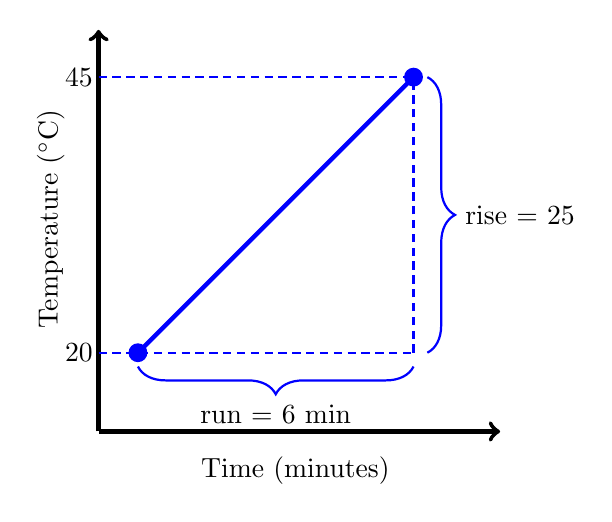
\begin{tikzpicture}
 
 % axis
  \draw[ultra thick, ->] (0, 0) -- (0, 5.1);
  \draw[ultra thick, ->] (0, 0) -- (5.1, 0);
\node[rotate=90] at (-0.8,2.5,-0.5) {Temperature ($^\circ$C)};
\node[] at (2.5,-0.5) {Time (minutes)};

  % grid
  %\draw[help lines, step = 0.5cm] (0, 0) grid (5, 5);

\draw[ultra thick, scale=0.5, domain=1:8,smooth,variable=\x, blue] plot ({\x},{1*\x+1});
\draw [draw=blue, fill=blue, thick] (.5,1) circle (3.0pt);
\draw [draw=blue, fill=blue, thick] (4,4.5) circle (3.0pt);
\draw [densely dashed, draw=blue, thick] (0,4.5) -- (4,4.5);
\draw [densely dashed, draw=blue, thick] (0,1) -- (.5,1);
\node[] at (-0.25,1) {20};
\node[] at (-0.25,4.5) {45};

%\draw [decorate,decoration={brace,amplitude=10pt, mirror},xshift=-0.5cm,yshift=0pt] (1,.75) -- (4.5,.75) node [black,below,xshift=-0.6cm] {run = $6$ min};

\draw[decoration={brace,mirror,raise=5pt, amplitude=10},decorate, draw=blue, thick] (.5,1) -- node[below=15pt] {run = 6 min} (4,1);
\draw [densely dashed, draw=blue, thick] (4,1) -- (4,4.5);

\draw[decoration={brace,mirror,raise=5pt, amplitude=10},decorate, draw=blue, thick] (4,1) -- node[right=15pt] {rise = 25} (4,4.5);
\draw [densely dashed, draw=blue, thick] (0,1) -- (4,1);
%\node[] at (.6,.6) {(12,20)};
%\node[] at (4,4.75) {(12,20)};
\end{tikzpicture}
\end{document}
